\documentclass{standalone}
\usepackage{tikz}
\usetikzlibrary{patterns, positioning}
\usepackage[sfdefault]{ClearSans} %% option 'sfdefault' activates Clear Sans as the default text font
\usepackage[T1]{fontenc}

\begin{document}
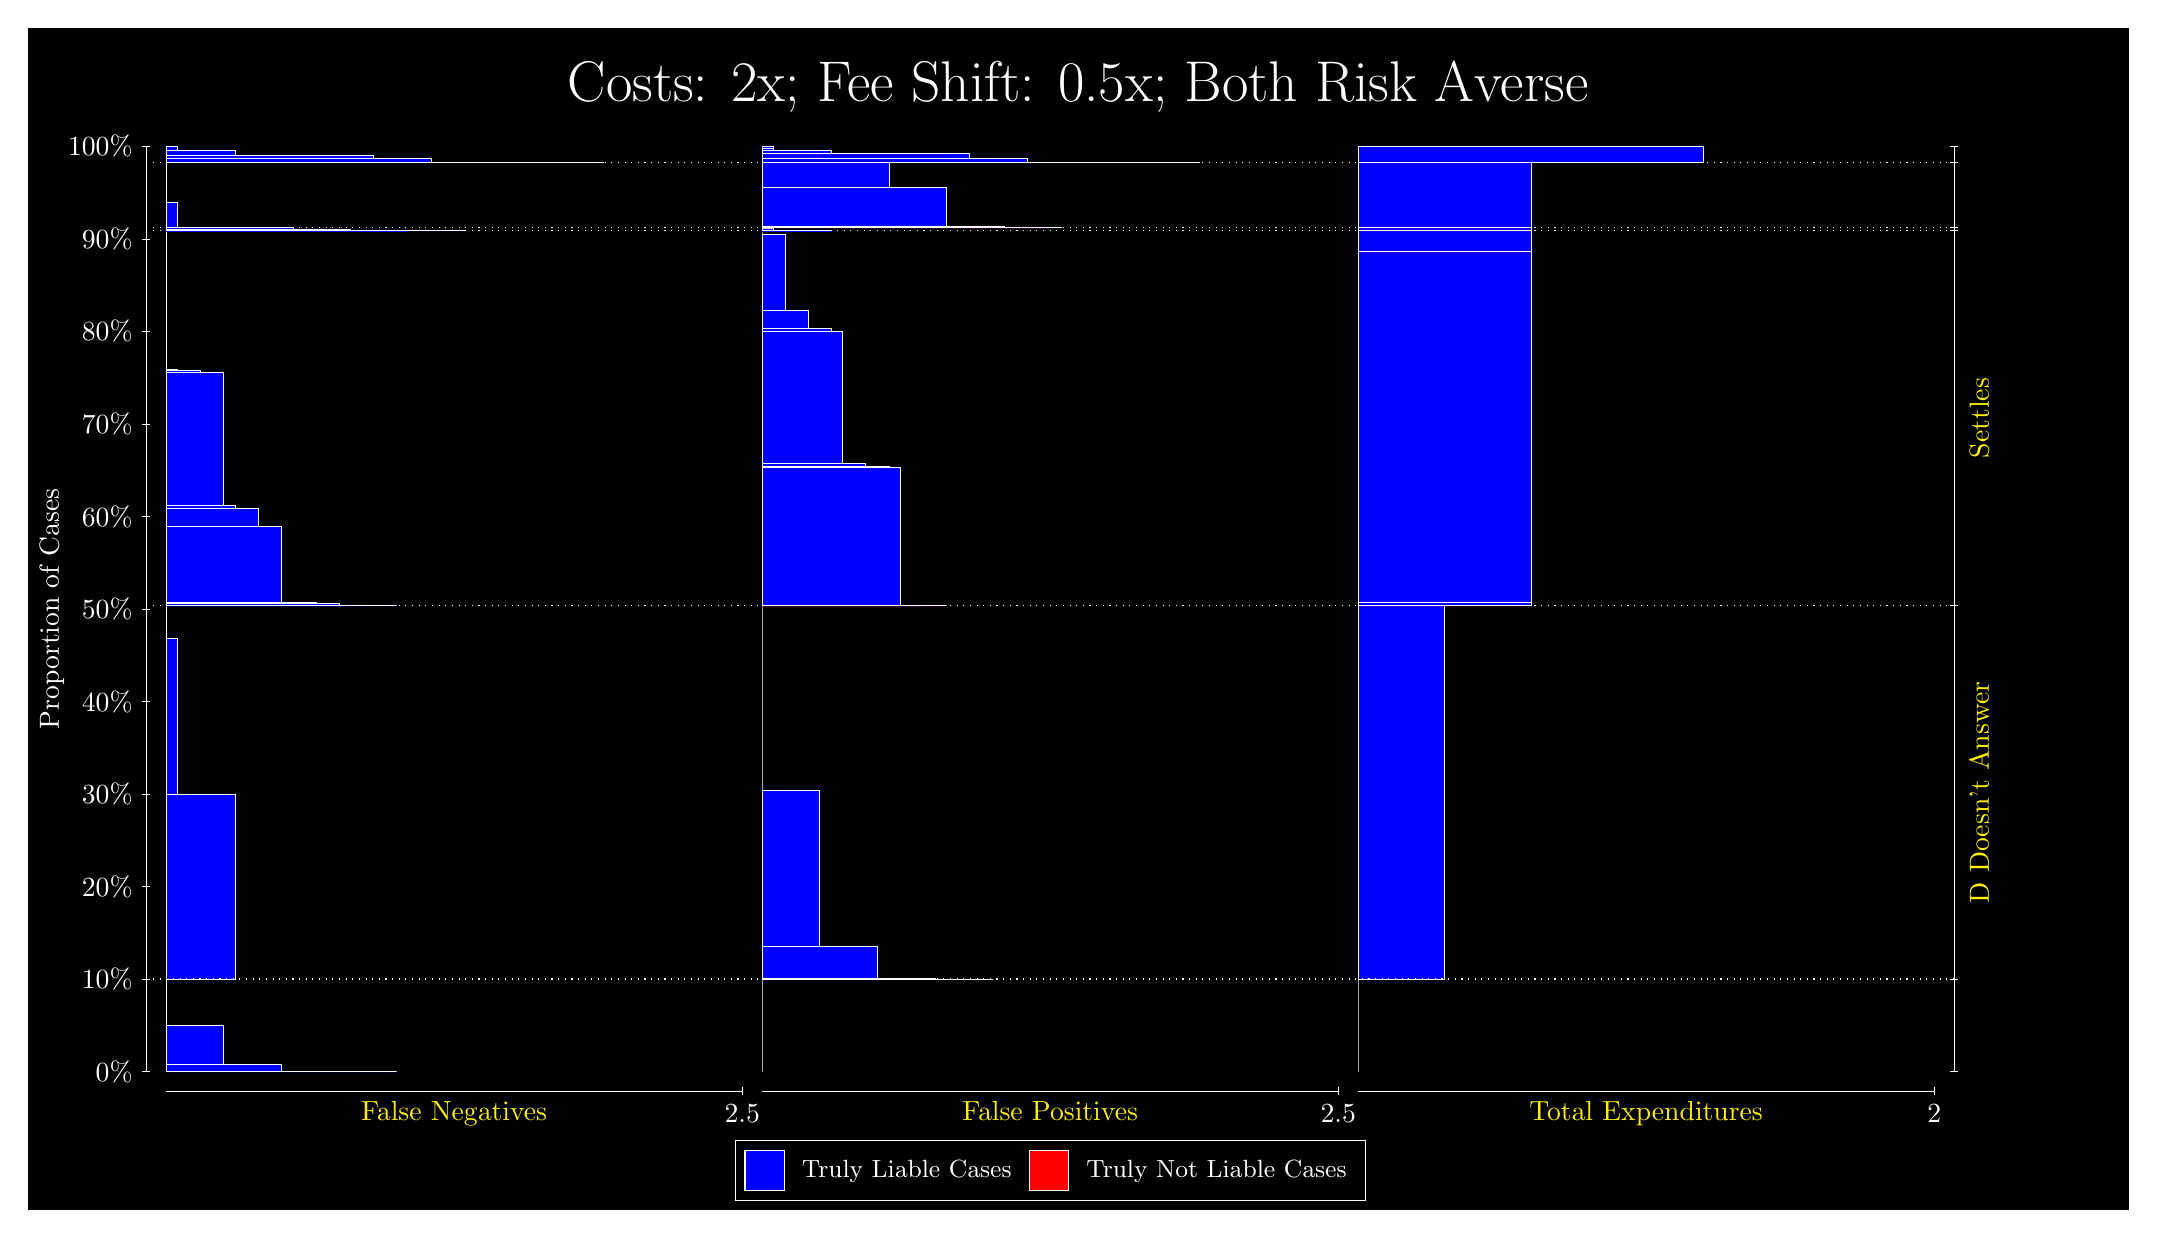
\begin{tikzpicture}
\draw[fill=black] (0,0) rectangle (26.667,15);
\draw[text=white] (0,13.5) rectangle (26.667,15) node[midway] {\huge Costs: 2x; Fee Shift: 0.5x; Both Risk Averse};
\draw[white, very thin] (1.5,1.75) -- (1.5,13.5);
\node[rotate=90, text=white, anchor=center] at (0.3, 7.625) {Proportion of Cases};
\draw[white, very thin] (1.45,1.75) -- (1.55,1.75);
\node[text=white, anchor=east] at (1.45, 1.75) {0\%};
\draw[white, very thin] (1.45,2.925) -- (1.55,2.925);
\node[text=white, anchor=east] at (1.45, 2.925) {10\%};
\draw[white, very thin] (1.45,4.1) -- (1.55,4.1);
\node[text=white, anchor=east] at (1.45, 4.1) {20\%};
\draw[white, very thin] (1.45,5.275) -- (1.55,5.275);
\node[text=white, anchor=east] at (1.45, 5.275) {30\%};
\draw[white, very thin] (1.45,6.45) -- (1.55,6.45);
\node[text=white, anchor=east] at (1.45, 6.45) {40\%};
\draw[white, very thin] (1.45,7.625) -- (1.55,7.625);
\node[text=white, anchor=east] at (1.45, 7.625) {50\%};
\draw[white, very thin] (1.45,8.8) -- (1.55,8.8);
\node[text=white, anchor=east] at (1.45, 8.8) {60\%};
\draw[white, very thin] (1.45,9.975) -- (1.55,9.975);
\node[text=white, anchor=east] at (1.45, 9.975) {70\%};
\draw[white, very thin] (1.45,11.15) -- (1.55,11.15);
\node[text=white, anchor=east] at (1.45, 11.15) {80\%};
\draw[white, very thin] (1.45,12.325) -- (1.55,12.325);
\node[text=white, anchor=east] at (1.45, 12.325) {90\%};
\draw[white, very thin] (1.45,13.5) -- (1.55,13.5);
\node[text=white, anchor=east] at (1.45, 13.5) {100\%};

\draw[white, very thin] (24.457,1.75) -- (24.457,13.5);
\draw[white, very thin] (24.407,1.75) -- (24.507,1.75);
\node[anchor=west] at (24.407, 1.75) {};
\draw[white, very thin] (24.407,2.9247) -- (24.507,2.9247);
\node[anchor=west] at (24.407, 2.9247) {};
\draw[white, very thin] (24.407,7.6677) -- (24.507,7.6677);
\node[anchor=west] at (24.407, 7.6677) {};
\draw[white, very thin] (24.407,12.429) -- (24.507,12.429);
\node[anchor=west] at (24.407, 12.429) {};
\draw[white, very thin] (24.407,12.467) -- (24.507,12.467);
\node[anchor=west] at (24.407, 12.467) {};
\draw[white, very thin] (24.407,13.297) -- (24.507,13.297);
\node[anchor=west] at (24.407, 13.297) {};
\draw[white, very thin] (24.407,13.5) -- (24.507,13.5);
\node[anchor=west] at (24.407, 13.5) {};

\draw[white, very thin, fill=blue] (1.75,1.75) rectangle (4.6775,1.75);
\draw[white, very thin, fill=blue] (1.75,1.75) rectangle (3.9457,1.7508);
\draw[white, very thin, fill=blue] (1.75,1.7508) rectangle (3.2138,1.844);
\draw[white, very thin, fill=blue] (1.75,1.844) rectangle (2.4819,2.3382);
\draw[white, very thin, fill=red] (1.75,2.3382) rectangle (1.75,2.3382);
\draw[white, very thin, fill=blue] (1.75,2.3382) rectangle (1.75,2.9247);
\draw[white, very thin, fill=blue] (1.75,2.9247) rectangle (2.6283,5.271);
\draw[white, very thin, fill=blue] (1.75,5.271) rectangle (1.8964,7.2565);
\draw[white, very thin, fill=red] (1.75,7.2565) rectangle (1.75,7.2565);
\draw[white, very thin, fill=blue] (1.75,7.2565) rectangle (1.75,7.6677);
\draw[white, very thin, fill=blue] (1.75,7.6677) rectangle (4.6775,7.6677);
\draw[white, very thin, fill=blue] (1.75,7.6677) rectangle (4.3848,7.6677);
\draw[white, very thin, fill=blue] (1.75,7.6677) rectangle (4.092,7.6677);
\draw[white, very thin, fill=blue] (1.75,7.6677) rectangle (3.9457,7.6993);
\draw[white, very thin, fill=blue] (1.75,7.6993) rectangle (3.6529,7.7101);
\draw[white, very thin, fill=blue] (1.75,7.7101) rectangle (3.3602,7.7119);
\draw[white, very thin, fill=blue] (1.75,7.7119) rectangle (3.2138,8.678);
\draw[white, very thin, fill=blue] (1.75,8.678) rectangle (2.921,8.9023);
\draw[white, very thin, fill=blue] (1.75,8.9023) rectangle (2.6283,8.94);
\draw[white, very thin, fill=blue] (1.75,8.94) rectangle (2.4819,10.629);
\draw[white, very thin, fill=blue] (1.75,10.629) rectangle (2.1891,10.662);
\draw[white, very thin, fill=blue] (1.75,10.662) rectangle (1.8964,10.668);
\draw[white, very thin, fill=red] (1.75,10.668) rectangle (1.75,10.668);
\draw[white, very thin, fill=blue] (1.75,10.668) rectangle (1.75,12.429);
\draw[white, very thin, fill=blue] (1.75,12.429) rectangle (5.5558,12.429);
\draw[white, very thin, fill=blue] (1.75,12.429) rectangle (4.8239,12.43);
\draw[white, very thin, fill=blue] (1.75,12.43) rectangle (4.092,12.443);
\draw[white, very thin, fill=blue] (1.75,12.443) rectangle (3.3602,12.467);
\draw[white, very thin, fill=blue] (1.75,12.467) rectangle (2.6283,12.467);
\draw[white, very thin, fill=red] (1.75,12.467) rectangle (1.75,12.467);
\draw[white, very thin, fill=blue] (1.75,12.467) rectangle (2.6283,12.471);
\draw[white, very thin, fill=blue] (1.75,12.471) rectangle (1.8964,12.788);
\draw[white, very thin, fill=red] (1.75,12.788) rectangle (1.75,12.788);
\draw[white, very thin, fill=blue] (1.75,12.788) rectangle (1.75,13.297);
\draw[white, very thin, fill=blue] (1.75,13.297) rectangle (7.3123,13.297);
\draw[white, very thin, fill=blue] (1.75,13.297) rectangle (6.5805,13.297);
\draw[white, very thin, fill=blue] (1.75,13.297) rectangle (5.8486,13.3);
\draw[white, very thin, fill=blue] (1.75,13.3) rectangle (5.1167,13.345);
\draw[white, very thin, fill=blue] (1.75,13.345) rectangle (4.8239,13.345);
\draw[white, very thin, fill=blue] (1.75,13.345) rectangle (4.3848,13.387);
\draw[white, very thin, fill=blue] (1.75,13.387) rectangle (4.092,13.387);
\draw[white, very thin, fill=blue] (1.75,13.387) rectangle (3.6529,13.388);
\draw[white, very thin, fill=blue] (1.75,13.388) rectangle (3.3602,13.389);
\draw[white, very thin, fill=blue] (1.75,13.389) rectangle (2.921,13.389);
\draw[white, very thin, fill=blue] (1.75,13.389) rectangle (2.6283,13.389);
\draw[white, very thin, fill=blue] (1.75,13.389) rectangle (2.6283,13.449);
\draw[white, very thin, fill=blue] (1.75,13.449) rectangle (1.8964,13.449);
\draw[white, very thin, fill=blue] (1.75,13.449) rectangle (1.8964,13.495);
\draw[white, very thin, fill=red] (1.75,13.495) rectangle (1.75,13.495);
\draw[white, very thin, fill=blue] (1.75,13.495) rectangle (1.75,13.5);
\draw[white, very thin, fill=red] (9.3189,1.75) rectangle (9.3189,1.75);
\draw[white, very thin, fill=blue] (9.3189,1.75) rectangle (9.3189,2.9247);
\draw[white, very thin, fill=red] (9.3189,2.9247) rectangle (12.246,2.9247);
\draw[white, very thin, fill=blue] (9.3189,2.9247) rectangle (12.246,2.9248);
\draw[white, very thin, fill=blue] (9.3189,2.9248) rectangle (11.515,2.9368);
\draw[white, very thin, fill=blue] (9.3189,2.9368) rectangle (10.783,3.3359);
\draw[white, very thin, fill=blue] (9.3189,3.3359) rectangle (10.051,5.3214);
\draw[white, very thin, fill=blue] (9.3189,5.3214) rectangle (9.3189,7.6677);
\draw[white, very thin, fill=red] (9.3189,7.6677) rectangle (11.661,7.6677);
\draw[white, very thin, fill=blue] (9.3189,7.6677) rectangle (11.661,7.6677);
\draw[white, very thin, fill=red] (9.3189,7.6677) rectangle (11.368,7.6677);
\draw[white, very thin, fill=blue] (9.3189,7.6677) rectangle (11.368,7.6677);
\draw[white, very thin, fill=red] (9.3189,7.6677) rectangle (11.075,7.6677);
\draw[white, very thin, fill=blue] (9.3189,7.6677) rectangle (11.075,9.4293);
\draw[white, very thin, fill=blue] (9.3189,9.4293) rectangle (10.929,9.435);
\draw[white, very thin, fill=blue] (9.3189,9.435) rectangle (10.636,9.4685);
\draw[white, very thin, fill=blue] (9.3189,9.4685) rectangle (10.344,11.157);
\draw[white, very thin, fill=blue] (9.3189,11.157) rectangle (10.197,11.195);
\draw[white, very thin, fill=blue] (9.3189,11.195) rectangle (9.9044,11.419);
\draw[white, very thin, fill=blue] (9.3189,11.419) rectangle (9.6116,12.385);
\draw[white, very thin, fill=blue] (9.3189,12.385) rectangle (9.4652,12.387);
\draw[white, very thin, fill=blue] (9.3189,12.387) rectangle (9.3189,12.429);
\draw[white, very thin, fill=red] (9.3189,12.429) rectangle (10.197,12.429);
\draw[white, very thin, fill=blue] (9.3189,12.429) rectangle (10.197,12.43);
\draw[white, very thin, fill=blue] (9.3189,12.43) rectangle (9.4652,12.454);
\draw[white, very thin, fill=blue] (9.3189,12.454) rectangle (9.3189,12.467);
\draw[white, very thin, fill=red] (9.3189,12.467) rectangle (13.125,12.467);
\draw[white, very thin, fill=blue] (9.3189,12.467) rectangle (13.125,12.467);
\draw[white, very thin, fill=blue] (9.3189,12.467) rectangle (12.393,12.481);
\draw[white, very thin, fill=blue] (9.3189,12.481) rectangle (11.661,12.977);
\draw[white, very thin, fill=blue] (9.3189,12.977) rectangle (10.929,13.294);
\draw[white, very thin, fill=blue] (9.3189,13.294) rectangle (10.197,13.297);
\draw[white, very thin, fill=red] (9.3189,13.297) rectangle (14.881,13.297);
\draw[white, very thin, fill=blue] (9.3189,13.297) rectangle (14.881,13.297);
\draw[white, very thin, fill=red] (9.3189,13.297) rectangle (14.149,13.297);
\draw[white, very thin, fill=blue] (9.3189,13.297) rectangle (14.149,13.297);
\draw[white, very thin, fill=red] (9.3189,13.297) rectangle (13.417,13.297);
\draw[white, very thin, fill=blue] (9.3189,13.297) rectangle (13.417,13.302);
\draw[white, very thin, fill=red] (9.3189,13.302) rectangle (12.686,13.302);
\draw[white, very thin, fill=blue] (9.3189,13.302) rectangle (12.686,13.349);
\draw[white, very thin, fill=blue] (9.3189,13.349) rectangle (11.954,13.408);
\draw[white, very thin, fill=red] (9.3189,13.408) rectangle (11.661,13.408);
\draw[white, very thin, fill=blue] (9.3189,13.408) rectangle (11.661,13.408);
\draw[white, very thin, fill=blue] (9.3189,13.408) rectangle (11.222,13.41);
\draw[white, very thin, fill=red] (9.3189,13.41) rectangle (10.929,13.41);
\draw[white, very thin, fill=blue] (9.3189,13.41) rectangle (10.929,13.41);
\draw[white, very thin, fill=blue] (9.3189,13.41) rectangle (10.49,13.41);
\draw[white, very thin, fill=blue] (9.3189,13.41) rectangle (10.197,13.451);
\draw[white, very thin, fill=red] (9.3189,13.451) rectangle (10.197,13.451);
\draw[white, very thin, fill=blue] (9.3189,13.451) rectangle (10.197,13.452);
\draw[white, very thin, fill=blue] (9.3189,13.452) rectangle (9.758,13.452);
\draw[white, very thin, fill=blue] (9.3189,13.452) rectangle (9.4652,13.479);
\draw[white, very thin, fill=blue] (9.3189,13.479) rectangle (9.4652,13.497);
\draw[white, very thin, fill=blue] (9.3189,13.497) rectangle (9.3189,13.5);
\draw[white, very thin, fill=red] (16.888,1.75) rectangle (16.888,1.75);
\draw[white, very thin, fill=blue] (16.888,1.75) rectangle (16.888,2.9247);
\draw[white, very thin, fill=red] (16.888,2.9247) rectangle (17.986,2.9247);
\draw[white, very thin, fill=blue] (16.888,2.9247) rectangle (17.986,7.6677);
\draw[white, very thin, fill=red] (16.888,7.6677) rectangle (19.083,7.6677);
\draw[white, very thin, fill=blue] (16.888,7.6677) rectangle (19.083,7.7128);
\draw[white, very thin, fill=red] (16.888,7.7128) rectangle (19.083,7.7128);
\draw[white, very thin, fill=blue] (16.888,7.7128) rectangle (19.083,12.161);
\draw[white, very thin, fill=red] (16.888,12.161) rectangle (19.083,12.161);
\draw[white, very thin, fill=blue] (16.888,12.161) rectangle (19.083,12.429);
\draw[white, very thin, fill=red] (16.888,12.429) rectangle (19.083,12.429);
\draw[white, very thin, fill=blue] (16.888,12.429) rectangle (19.083,12.467);
\draw[white, very thin, fill=red] (16.888,12.467) rectangle (19.083,12.467);
\draw[white, very thin, fill=blue] (16.888,12.467) rectangle (19.083,13.297);
\draw[white, very thin, fill=red] (16.888,13.297) rectangle (21.279,13.297);
\draw[white, very thin, fill=blue] (16.888,13.297) rectangle (21.279,13.5);
\draw[white, dotted] (1.5,2.9247) -- (24.457,2.9247);
\draw[white, dotted] (1.5,7.6677) -- (24.457,7.6677);
\draw[white, dotted] (1.5,12.429) -- (24.457,12.429);
\draw[white, dotted] (1.5,12.467) -- (24.457,12.467);
\draw[white, dotted] (1.5,13.297) -- (24.457,13.297);
\draw[white, very thin] (1.75,1.5) -- (9.0689,1.5);
\node[text=yellow, anchor=north] at (5.4094, 1.5) {False Negatives};
\draw[white, very thin] (9.0689,1.45) -- (9.0689,1.55);
\node[text=white, anchor=north] at (9.0689, 1.45) {2.5};

\draw[white, very thin] (9.3189,1.5) -- (16.638,1.5);
\node[text=yellow, anchor=north] at (12.978, 1.5) {False Positives};
\draw[white, very thin] (16.638,1.45) -- (16.638,1.55);
\node[text=white, anchor=north] at (16.638, 1.45) {2.5};

\draw[white, very thin] (16.888,1.5) -- (24.207,1.5);
\node[text=yellow, anchor=north] at (20.547, 1.5) {Total Expenditures};
\draw[white, very thin] (24.207,1.45) -- (24.207,1.55);
\node[text=white, anchor=north] at (24.207, 1.45) {2};


\node[text=yellow, centered, rotate=90] at (24.777, 5.2962) {D Doesn't Answer};
\node[text=yellow, centered, rotate=90] at (24.777, 10.049) {Settles};




\draw (12.978300999999998,1.5) node[draw=none] (baseCoordinate) {};
\begin{scope}[align=center]
        \matrix[scale=0.5, draw=white, below=0.5cm of baseCoordinate, nodes={draw}, column sep=0.1cm]{
            \node[rectangle, draw, minimum width=0.5cm, minimum height=0.5cm, fill=blue] {}; &
            \node[draw=none, font=\small, text=white] (B) {Truly Liable Cases}; &
            \node[rectangle, draw, minimum width=0.5cm, minimum height=0.5cm, fill=red] {}; &
            \node[draw=none, font=\small, text=white] (B) {Truly Not Liable Cases}; \\
            };
\end{scope}

\end{tikzpicture}
\end{document}